\documentclass[11pt, a4paper, openany, oneside]{book}
\raggedbottom

\usepackage{import}
% Header file containing style definitions

% --- Essential Packages ---
\usepackage[utf8]{inputenc}
\usepackage[T1]{fontenc}
\usepackage[english]{babel}
\usepackage{geometry}
\geometry{a4paper, margin=1in} % Professional tight spacing

% --- Typography & Colors ---
\usepackage{lmodern} % scalable fonts
\usepackage{microtype} % Better spacing
\usepackage[table]{xcolor}

% Define Theme Colors (Blues / Purples / Greys)
\definecolor{hfblue}{HTML}{2D31FA}      % Hugging Face-ish Blue
\definecolor{hfpurple}{HTML}{6B4D8F}    % Subtle Purple
\definecolor{hfgrey}{HTML}{F3F4F6}      % Light Grey for backgrounds
\definecolor{codebg}{HTML}{F5F5F5}
\definecolor{darkgrey}{HTML}{333333}

% --- Graphics & Diagrams ---
\usepackage{graphicx}
\usepackage{tikz}
\usepackage{float}
\usetikzlibrary{shapes, arrows, positioning, shadows, trees, calc}
% \usepackage{smartdiagram}
% \usesmartdiagramlibrary{additions}
\usepackage{pgfplots}
\pgfplotsset{compat=1.18}
\usepackage{pifont} % For symbols

% --- Boxes and Highlights ---
\usepackage{tcolorbox}
\tcbuselibrary{breakable}

% Definition Box
\newtcolorbox{definitionbox}[1]{
  colback=blue!5!white,
  colframe=hfblue,
  fonttitle=\bfseries,
  title=Definition: #1,
  boxrule=0.5mm,
  sharp corners,
  breakable
}

% Example Box
\newtcolorbox{examplebox}[1]{
  colback=green!5!white,
  colframe=green!60!black,
  fonttitle=\bfseries,
  title=Example: #1,
  boxrule=0.5mm,
  breakable
}

% Tip Box
\newtcolorbox{tipbox}{
  colback=yellow!10!white,
  colframe=orange!80!black,
  fonttitle=\bfseries,
  title=Tip,
  boxrule=0.5mm,
  breakable
}

% Warning Box
\newtcolorbox{warningbox}{
  colback=red!5!white,
  colframe=red!75!black,
  fonttitle=\bfseries,
  title=Warning,
  boxrule=0.5mm,
  breakable
}

% --- Code Listings ---
\usepackage{listings}
\lstset{
    language=Python,
    basicstyle=\ttfamily\small,
    backgroundcolor=\color{codebg},
    keywordstyle=\color{hfblue}\bfseries,
    stringstyle=\color{green!50!black},
    commentstyle=\color{gray}\itshape,
    numberstyle=\tiny\color{gray},
    numbers=left,
    stepnumber=1,
    frame=single,
    rulecolor=\color{lightgray},
    breaklines=true,
    captionpos=b,
    showstringspaces=false
}

% --- Navigation ---
\usepackage{hyperref}
\hypersetup{
    colorlinks=true,
    linkcolor=hfblue,
    filecolor=magenta,      
    urlcolor=hfpurple,
    pdftitle={Hugging Face Guide},
    pdfpagemode=FullScreen,
}

% --- Header/Footer ---
\usepackage{fancyhdr}
\setlength{\headheight}{14pt}
\pagestyle{fancy}
\fancyhf{}
\fancyhead[L]{\nouppercase{\leftmark}}
\fancyhead[R]{\thepage}

\usepackage{fancyhdr}

% Define Footer
\pagestyle{fancy}
\fancyhf{} % Clear defaults
\fancyfoot[C]{Mausam Kar -- Full Stack Developer}
\fancyfoot[R]{\thepage}
\renewcommand{\headrulewidth}{0pt} % Remove header line

% Apply to Chapter pages (plain style) as well
\fancypagestyle{plain}{
    \fancyhf{}
    \fancyfoot[C]{Mausam Kar -- Full Stack Developer}
    \fancyfoot[R]{\thepage}
    \renewcommand{\headrulewidth}{0pt}
}

\begin{document}
\let\cleardoublepage\clearpage

% --- Front Matter ---
\frontmatter

% Custom Title Page
\begin{titlepage}
    \begin{tikzpicture}[remember picture, overlay]
        % Background Color
        \fill[hfblue] (current page.south west) rectangle (current page.north east);
        
        % Decorative Stripe
        \fill[hfpurple] (current page.south west) -- (current page.north west) -- ([xshift=3cm]current page.north west) -- ([xshift=3cm]current page.south west) -- cycle;
        
        % Title Text
        \node[anchor=north west, inner sep=0, text width=14cm] at ([xshift=4cm, yshift=-5cm]current page.north west) {
            {\fontsize{40}{50}\selectfont \bfseries \color{white} Project Report: \\ Multilingual Translator} \\[1cm]
            {\fontsize{20}{25}\selectfont \itshape \color{yellow!80!black} Architecture, Setup, and Usage Guide}
        };
        
        % Author Name
        \node[anchor=south west, inner sep=0] at ([xshift=4cm, yshift=4cm]current page.south west) {
            {\fontsize{18}{22}\selectfont \bfseries \color{white} Technical Documentation}
        };

        % TikZ Smiley Logo
        \node[anchor=south east, opacity=0.3] at ([xshift=-1cm, yshift=1cm]current page.south east) {
             \begin{tikzpicture}
                \fill[white] (0,0) circle (2cm);
                \fill[hfblue] (-0.7,0.5) circle (0.3cm); 
                \fill[hfblue] (0.7,0.5) circle (0.3cm);
                \draw[hfblue, line width=2mm] (-1,-0.5) arc (180:360:1cm);
                \node at (0, -2.5) {\bfseries \Huge App};
            \end{tikzpicture}
        };
    \end{tikzpicture}
\end{titlepage}

\tableofcontents
% Lists removed per user request
% \tableofcontents only

% --- Main Content ---
\mainmatter

\chapter{Project Overview \& Architecture}

\section{Introduction}
In today's interconnected world, language barriers remain a significant challenge. The **Multilingual Translator \& Summariser** is an AI-powered application designed to bridge this gap. It allows users to input text in \textit{any} language, automatically translates it into English, and then provides a concise summary of the content.

\section{Problem \& Solution}
\begin{itemize}
    \item \textbf{The Problem:} Information Overload. Valuable documents (news, research, user feedback) are often available only in local languages and are too long to digest quickly.
    \item \textbf{The Solution:} A single-click pipeline.
    \begin{enumerate}
        \item \textbf{Translate:} Convert local language `X` to English using \texttt{NLLB-200}.
        \item \textbf{Summarize:} Condense the English text using \texttt{BART-Large}.
        \item \textbf{Present:} Display both outputs in a clean, reactive Web UI.
    \end{enumerate}
\end{itemize}

\section{System Design}
The system follows a modular architecture, separating the core AI logic from the user interface.

\begin{figure}[H]
    \centering
    % Resize box ensures it fits exactly within the page margins
    \resizebox{\textwidth}{!}{
    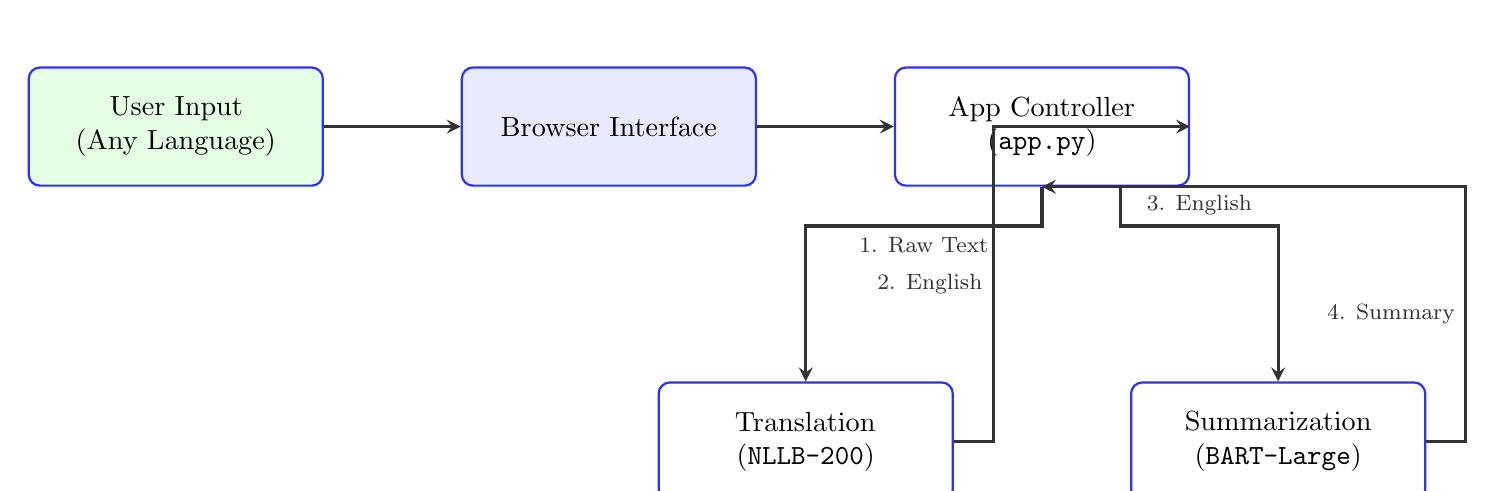
\begin{tikzpicture}[
        node distance=4cm,
        auto,
        block/.style={rectangle, draw=hfblue, thick, fill=white, text width=3.5cm, align=center, rounded corners, minimum height=1.5cm},
        line/.style={draw, very thick, color=darkgrey, ->, >=stealth},
        label/.style={midway, fill=white, font=\footnotesize, text=darkgrey}
    ]
        % Layout: User -> UI -> App (Horizontal)
        \node [block, fill=green!10] (user) {User Input \\ (Any Language)};
        \node [block, right of=user, node distance=5.5cm, fill=hfblue!10] (ui) {Browser Interface};
        \node [block, right of=ui, node distance=5.5cm] (app) {App Controller \\ (\texttt{app.py})};
        
        % Services (Below App)
        \node [block, below of=app, xshift=-3cm, node distance=4cm] (trans) {Translation \\ (\texttt{NLLB-200})};
        \node [block, below of=app, xshift=3cm, node distance=4cm] (summ) {Summarization \\ (\texttt{BART-Large})};

        % Connections
        \draw [line] (user) -- (ui);
        \draw [line] (ui) -- (app);
        
        % App to Services (Orthogonal Paths)
        % App -> Trans
        \draw [line] (app.south) -- ++(0,-0.5) -| node[label, pos=0.25] {1. Raw Text} (trans.north);
        % Trans -> App
        \draw [line] (trans.east) -- ++(0.5,0) |- node[label, pos=0.25] {2. English} (app.east);
        
        % App -> Summ
        % We connect App East to Summ North (via path)
        % Actually, let's go from App South (shifted) to Summ North
        \draw [line] (app.south) ++(1,0) -- ++(0,-0.5) -| node[label, pos=0.25] {3. English} (summ.north);
        
        % Summ -> App
        % Summ East to App East?
        \draw [line] (summ.east) -- ++(0.5,0) |- node[label, pos=0.25] {4. Summary} (app.south);
        
    \end{tikzpicture}
    }
    \caption{Data Flow Architecture}
\end{figure}

\section{Model Decisions}
\begin{description}
    \item[Translation Model:] We selected `facebook/nllb-200-distilled-600M`.
    \begin{itemize}
        \item \textbf{Pros:} Supports 200+ languages, high accuracy, reasonable size (1.2GB).
        \item \textbf{Why Distilled?} The full model is 54GB, which is impossible to run on consumer hardware. The distilled version offers 90\% of the performance at 2\% of the size.
    \end{itemize}
    
    \item[Summarization Model:] We selected `facebook/bart-large-cnn`.
    \begin{itemize}
        \item \textbf{Pros:} State-of-the-art for abstractive summarization on news articles.
        \item \textbf{Why CNN?} It was fine-tuned on the CNN/DailyMail dataset, making it excellent for understanding journalistic and factual content.
    \end{itemize}
\end{description}

% % This chapter has been merged into 01_overview.tex to reduce blank space.
 % Merged into overview
\chapter{Installation \& Setup}

This guide assumes you are running on Windows, but the commands are similar for Mac/Linux. We will cover the installation of Python, the creation of a virtual environment, and the installation of the machine learning dependencies.

\section{Prerequisites}
Before diving in, ensure you have the following installed on your system:
\begin{enumerate}
    \item \textbf{Python 3.8+}: Hugging Face libraries require a modern Python version. Verification: \texttt{python --version}.
    \item \textbf{Git}: Standard for version control, useful for cloning the repository.
    \item \textbf{Internet Connection}: To download model weights. The models (\texttt{NLLB-200} and \texttt{BART-Large}) are approx 2-3 GB combined.
    \item \textbf{Hardware:} A GPU (NVIDIA GTX 1650 or better) is recommended for fast inference. If you use a CPU, expect delays of 10-15 seconds per request.
\end{enumerate}

\section{Step-by-Step Installation}

\subsection{1. Clone the Repository}
Open your terminal (PowerShell or Command Prompt) and navigate to your workspace.
\begin{lstlisting}[language=bash]
# Clone the project code
git clone https://github.com/your-repo/multilingual-translator.git

# Enter the directory
cd multilingual-translator
\end{lstlisting}

\subsection{2. Create a Virtual Environment}
It is "best practice" to isolate dependencies so they don't conflict with other projects.
\begin{lstlisting}[language=bash]
# Create the environment named 'venv'
python -m venv venv

# Activate it (Windows)
# Your prompt should change to start with (venv)
venv\Scripts\activate

# Activate it (Linux/Mac)
source venv/bin/activate
\end{lstlisting}

\subsection{3. Install Dependencies}
We rely on \texttt{torch}, \texttt{transformers}, and \texttt{gradio}.
\begin{lstlisting}[language=bash]
# Upgrade pip first to avoid errors
pip install --upgrade pip

# Install dependencies from the file
pip install -r requirements.txt
\end{lstlisting}

\section{GPU Configuration (Optional but Recommended)}
Standard \texttt{pip install torch} usually installs the CPU version. To enable GPU support:

\begin{enumerate}
    \item Check your CUDA version (open NVIDIA Control Panel or run \texttt{nvidia-smi}).
    \item Go to \url{https://pytorch.org/get-started/locally/}.
    \item Copy the command for your version. For example (CUDA 11.8):
\end{enumerate}

\begin{lstlisting}[language=bash]
pip install torch torchvision torchaudio --index-url https://download.pytorch.org/whl/cu118
\end{lstlisting}

\section{Directory Structure Verification}
After installation, your project folder should look like this:
\begin{lstlisting}[language=bash]
multilingual-translator/
|-- venv/                # Virtual Environment (do not touch)
|-- src/
|   |-- __init__.py
|   |-- translation.py   # Translation Logic
|   |-- summarization.py # Summarization Logic
|-- app.py               # Main Entry Point
|-- requirements.txt     # Dependency List
|-- README.md            # Quick Start Guide
\end{lstlisting}

\begin{warningbox}
Do not commit the \texttt{venv/} folder to Git! It is specific to your machine and very large. Use a \texttt{.gitignore} file to exclude it.
\end{warningbox}

\section{Troubleshooting Common Issues}
\begin{itemize}
    \item \textbf{Error: "Module not found"}: Ensure you activated the virtual environment before running the app.
    \item \textbf{Error: "Torch not compiled with CUDA enabled"}: You installed the CPU version of Torch. Uninstall it (\texttt{pip uninstall torch}) and reinstall the GPU version using the command above.
    \item \textbf{Slow Performance}: If the translation takes >30 seconds, you are likely running on CPU. This is expected for large models like NLLB-200.
    \item \textbf{Download Fails}: These models are hosted on Hugging Face Hub. If you have a firewall, you might need to use a proxy or check your internet connection.
\end{itemize}

\chapter{Usage Manual}

This chapter guides you through running the application and understanding the user interface.

\section{Running the Application}
With your environment active, run the following command in your terminal:
\begin{lstlisting}[language=bash]
python app.py
\end{lstlisting}

\subsection{Startup Logs}
You should see output similar to the following. Note the model loading times:
\begin{verbatim}
Initializing AI Services...
Loading Translation Model: facebook/nllb-200-distilled-600M...
(This may take 10-20 seconds on first run to download 1.2GB)
Loading Summarization Model: facebook/bart-large-cnn...
(This may take 10-15 seconds to download 1.6GB)
Services loaded successfully.
Running on local URL:  http://127.0.0.1:7860
\end{verbatim}

Open your browser (Chrome/Edge/Firefox) and navigate to \url{http://127.0.0.1:7860}.

\section{Interface Overview}
The User Interface (UI) is built with Gradio and consists of three main sections:

\begin{figure}[H]
    \centering
    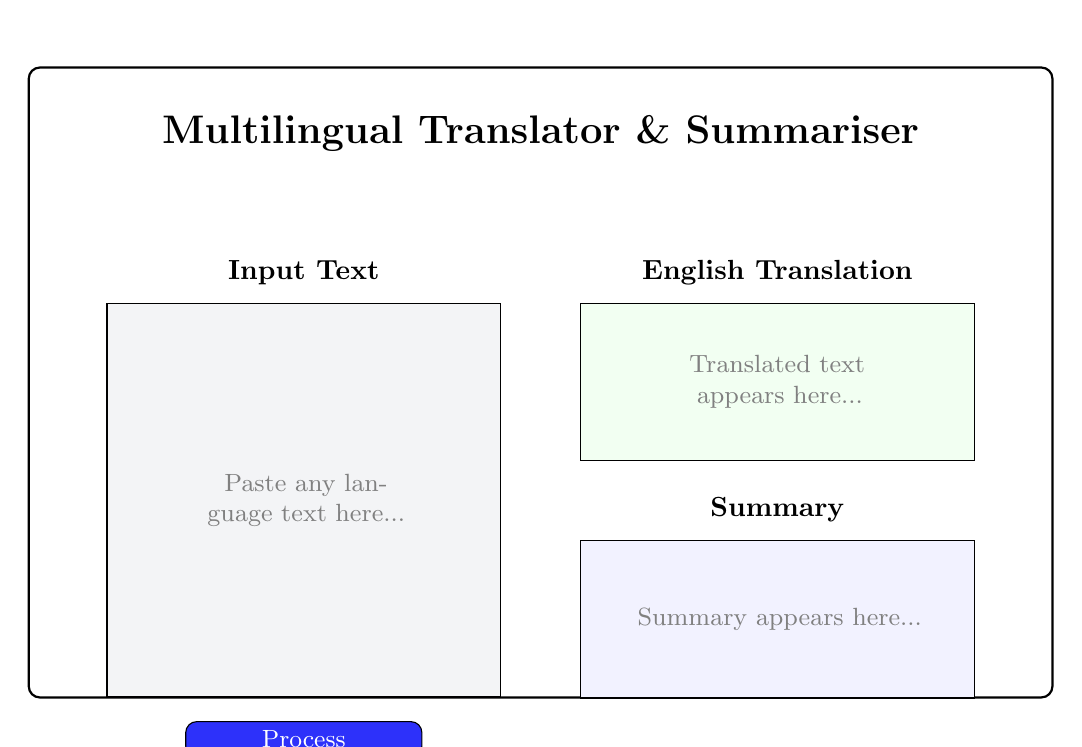
\begin{tikzpicture}[font=\small]
        % Window frame (Wider)
        \node[draw, thick, rounded corners, minimum width=13cm, minimum height=8cm, fill=white] (window) {};
        
        % Header inside window
        \node[below=0.5cm of window.north, font=\bfseries\Large] {Multilingual Translator \& Summariser};
        
        % Left Column: Input
        \node[draw, fill=hfgrey, minimum width=5cm, minimum height=5cm, below right=3cm and 1cm of window.north west] (input) {};
        \node[above=0.1cm of input, font=\bfseries] {Input Text};
        \node[gray, text width=4cm, align=center] at (input.center) {Paste any language text here...};
        
        % Button
        \node[draw, fill=hfblue, text=white, minimum width=3cm, rounded corners, below=0.3cm of input] {Process};

        % Right Column: Outputs
        % Output 1
        \node[draw, fill=green!5, minimum width=5cm, minimum height=2cm, below left=3cm and 1cm of window.north east] (out1) {};
        \node[above=0.1cm of out1, font=\bfseries] {English Translation};
        \node[gray, text width=4cm, align=center] at (out1.center) {Translated text appears here...};

        % Output 2
        \node[draw, fill=blue!5, minimum width=5cm, minimum height=2cm, below=1cm of out1] (out2) {};
        \node[above=0.1cm of out2, font=\bfseries] {Summary};
        \node[gray, text width=4cm, align=center] at (out2.center) {Summary appears here...};
    \end{tikzpicture}
    \caption{UI Layout Mockup}
\end{figure}

\section{Step-by-Step Workflow}
\begin{enumerate}
    \item \textbf{Input Field:} Copy and paste any text into the large box on the left. The model handles over 200 languages (Spanish, Hindi, French, Japanese, etc.).
    \item \textbf{Process Button:} Click the "Process" button. The button will show a loading spinner while the GPU processes the request.
    \item \textbf{Outputs:}
    \begin{itemize}
        \item \textbf{Top Right (Translation):} The system first translates the input into English. This preserves the full detail of the original text.
        \item \textbf{Bottom Right (Summary):} The system then reads the English translation and creates a 2-3 sentence abstractive summary.
    \end{itemize}
\end{enumerate}

\section{Example Scenarios}

\subsection{Scenario 1: News Article (Hindi)}
\begin{itemize}
    \item \textbf{Input:} "Bharat ek vishaal desh hai..." (A long paragraph about India's geography).
    \item \textbf{Action:} User clicks Process.
    \item \textbf{Translation:} "India is a vast country..."
    \item \textbf{Summary:} "India is geographically diverse with ancient culture."
\end{itemize}

\subsection{Scenario 2: Tech Review (French)}
\begin{itemize}
    \item \textbf{Input:} "Ce nouvel ordinateur portable est incroyablement rapide mais la batterie..."
    \item \textbf{Translation:} "This new laptop is incredibly fast but the battery..."
    \item \textbf{Summary:} "The laptop has excellent performance but poor battery life."
\end{itemize}

\begin{warningbox}
The first request might be slow (10-20 seconds) as the computer "warms up" the models (JIT Compilation). Subsequent requests will be much faster.
\end{warningbox}

\section{Advanced Customization}
Want to change the models? You can modify `src/translation.py`:

\subsection{Using a Smaller Model}
If you are on an older laptop, switch to the 600M distilled version or even the 1.3B version if you have more RAM.
\begin{lstlisting}[language=Python]
# In src/translation.py
self.model_name = "facebook/nllb-200-distilled-600M" # Fast
# self.model_name = "facebook/nllb-200-3.3B"         # Very Slow, More Accurate
\end{lstlisting}

\subsection{Changing the Summary Style}
You can make the summary bullet-pointed by editing `src/summarization.py`:
\begin{lstlisting}[language=Python]
# In src/summarization.py
def summarize(self, text):
    prompt = f"Summarize this in bullet points: {text}"
    # ... rest of code
\end{lstlisting}

\chapter{Code Implementation Details}

This chapter provides a deep dive into the implementation. We use object-oriented programming to keep the codebase modular and testable.

\section{Translation Service}
File: \texttt{src/translation.py}

The `TranslationService` class encapsulates the complexity of the NLLB model. 

\begin{lstlisting}[language=Python, caption=Initializing NLLB]
class TranslationService:
    def __init__(self, model_name="facebook/nllb-200-distilled-600M"):
        # We check for GPU availability automatically
        self.device = 0 if torch.cuda.is_available() else -1
        
        print(f"Loading Translation Model: {model_name}...")
        self.tokenizer = AutoTokenizer.from_pretrained(model_name)
        self.model = AutoModelForSeq2SeqLM.from_pretrained(model_name)
        
        if self.device == 0:
            self.model = self.model.to("cuda")
\end{lstlisting}

\subsection{Handling Multilingual Inputs}
The core challenge with NLLB is that it requires a "Forced BOS Token" (Beginning of Sentence) to know which language to translate \textit{into}.

\begin{lstlisting}[language=Python, caption=Forcing English Output]
    def translate(self, text, target_lang="eng_Latn"):
        if not text: return ""

        # 1. Tokenize Input
        inputs = self.tokenizer(text, return_tensors="pt", padding=True)
        if self.device == 0:
            inputs = {k: v.to("cuda") for k, v in inputs.items()}

        # 2. Force Target Language Token
        # "eng_Latn" is the NLLB code for English
        forced_bos = self.tokenizer.convert_tokens_to_ids(target_lang)
        
        # 3. Generate
        with torch.no_grad():
            tokens = self.model.generate(
                **inputs, 
                forced_bos_token_id=forced_bos, 
                max_length=512
            )
            
        # 4. Decode
        return self.tokenizer.batch_decode(tokens, skip_special_tokens=True)[0]
\end{lstlisting}

\section{Summarization Service}
File: \texttt{src/summarization.py}

The summarizer is simpler because we leverage the Hugging Face `pipeline` abstraction.

\begin{lstlisting}[language=Python]
class SummarizationService:
    def __init__(self):
        # Pipelines handle tokenization, device placement, and decoding internally
        self.summarizer = pipeline("summarization", model="facebook/bart-large-cnn")

    def summarize(self, text):
        # We set tight constraints on length to ensure concise outputs
        result = self.summarizer(
            text, 
            max_length=130,  # Max summary length
            min_length=30,   # Min summary length
            do_sample=False  # Deterministic output
        )
        return result[0]['summary_text']
\end{lstlisting}

\section{The Application Controller}
File: \texttt{app.py}

Finally, we tie everything together. 

\begin{figure}[H]
    \centering
    
\begin{tikzpicture}[node distance=3cm]
        \node[font=\bfseries, align=center, text width=2cm] (start) {User Click};
        \node[right of=start, draw, align=center, text width=3.5cm] (t) {TranslationService \\ .translate()};
        \node[right of=t, draw, align=center, text width=3.5cm, xshift=1.5cm] (s) {SummarizationService \\ .summarize()};
        \node[right of=s, align=center, text width=2cm, xshift=0.5cm] (end) {Update UI};
        
        \draw[->, thick] (start) -- (t);
        \draw[->, thick] (t) -- (s);
        \draw[->, thick] (s) -- (end);
    \end{tikzpicture}
    \caption{Execution Flow}
\end{figure}

The \texttt{app.py} script initializes these services once (globally) so they don't reload on every request, which would be very slow.


\end{document}
